\documentclass{exam}
\usepackage{graphicx} 

%Format Header and footer
\pagestyle{headandfoot}
\header{\footnotesize Klass:\\Namn:}{\Large\textbf{Prov: Grundläggande kemi}}{\footnotesize Nak2\\2024}
\headrule
\footrule
\setlength{\columnsep}{0.25cm}
%\setlength{\columnseprule}{1pt}
\footer{}{Sida \thepage}{}
%\extrafootheight{-2cm}

\begin{document}

\section*{Instruktioner}
Svara på följande frågor. Flera alternativ kan vara korrekta, detta är tydligt angivet i frågan när det är fallet. Svara kortfattat.

\subsection*{Poäng}
Antalet poäng är markerat för varje fråga. Totalt \textbf{14 frågor} och \textbf{16 poäng}.\\ \textit{För godkänt resultat krävs 9 poäng.}

\section*{Frågor}

\hrule 
\vspace{5mm} 
\begin{questions}

\question Vilka av följande är \textbf{subatoma partiklar}? (Flera svar kan vara korrekta) (1 poäng)
\vspace{2mm} 
\begin{checkboxes}
    \choice Proton
    \choice Jon
    \choice Neutron
    \choice Legering
\end{checkboxes}

\vspace{5mm} 
\hrule 
\vspace{5mm} 

\question Vilken \textbf{laddning} har följande partiklar? (1 poäng)
\begin{itemize}
     \vspace{5mm} 
     \item \textbf{Elektron}
     \vspace{5mm} 
     \item \textbf{Neutron}
    \vspace{5mm} 
     \item \textbf{Proton}
     \vspace{5mm} 
\end{itemize}

\vspace{5mm} 
\hrule 
\vspace{5mm} 

\question Vilket alternativ beskriver bäst en \textbf{isotop}? (1 poäng)
\vspace{2mm} 
\begin{checkboxes}
    \choice Två atomer med samma antal neutroner men olika antal elektroner
    \choice Två atomer med samma antal protoner men olika antal elektroner
    \choice Två atomer med samma antal protoner men olika antal neutroner
    \choice Två atomer med samma antal neutroner men olika antal protoner
\end{checkboxes}

\vspace{5mm} 
\hrule 
\vspace{5mm} 

\question Markera i bilden. (1 poäng)

\begin{center}
    \begin{minipage}{0.4\textwidth}
        
\includegraphics[width=80pt]{image.png}
    \end{minipage}
    \begin{minipage}{0.5\textwidth}
        \begin{itemize}
            \item \textbf{Masstal}
            \item \textbf{Atomnummer}
        \end{itemize}
    \end{minipage}
\end{center}



\break
% Inkluderade nya frågor här
\question Vad bestämmer vilket \textbf{grundämne} en atom tillhör? (1 poäng)
\vspace{2mm}
\begin{checkboxes}
    \choice Antalet protoner i atomkärnan
    \choice Antalet neutroner i atomkärnan
    \choice Antalet elektroner i atomen
    \choice Elektronernas fördelning i elektronskal
\end{checkboxes}

\vspace{5mm} 
\hrule 
\vspace{5mm} 

\question Vilka av följande påståenden om \textbf{valenselektroner} är sanna? (Flera svar kan vara korrekta) (1 poäng)
\vspace{2mm}
\begin{checkboxes}
    \choice Valenselektroner finns i atomens yttersta skal
    \choice Valenselektroner påverkar atomens reaktivitet
    \choice Valenselektroner finns i alla elektronskal
    \choice Atomer med fyllda valensskal är ofta mindre reaktiva
\end{checkboxes}

\vspace{5mm} 
\hrule 
\vspace{5mm} 

\question Vilka av följande påståenden om \textbf{fusion} är korrekta? (Flera svar kan vara korrekta) (1 poäng)
\vspace{2mm}
\begin{checkboxes}
    \choice Fusion innebär att två lättare atomkärnor slås ihop
    \choice Fusion sker naturligt i stjärnor
    \choice Fusion används i kärnkraftverk på jorden
    \choice Fusion frigör enorma mängder energi
\end{checkboxes}

\vspace{5mm} 
\hrule 
\vspace{5mm} 

\question Vilken typ av \textbf{blandning} kan man se de olika beståndsdelarna i? (1 poäng)
\vspace{2mm}
\begin{checkboxes}
    \choice Homogen blandning
    \choice Heterogen blandning
    \choice Legering
    \choice Molekylär blandning
\end{checkboxes}

\vspace{5mm} 
\hrule 
\vspace{5mm} 

\question Vad innebär ett \textbf{elektronpar} i kemisk bindning? (1 poäng)
\begin{checkboxes}
\choice Två elektroner som delas mellan atomer i en kovalent bindning.
\choice Två elektroner som befinner sig i atomens kärna.
\choice Två elektroner som tillhör en och samma jon.
\choice Två elektroner som flyttar från en atom till en annan vid en jonbindning.
\end{checkboxes}

\break

\question Vilket av följande alternativ beskriver bäst en \textbf{ädelgas}? (1 poäng)
\vspace{2mm} 
\begin{checkboxes}
\choice En atom som har ett fullt yttersta elektronskal och därmed är kemiskt stabil.
\choice En atom som saknar elektroner i sitt yttersta elektronskal och därmed är mycket reaktiv.
\choice En atom som lätt bildar jonföreningar.
\choice En atom som har lika många protoner som elektroner.
\end{checkboxes}

\vspace{5mm} 
\hrule 
\vspace{5mm} 

\question Beskriv kortfattat skillnaden mellan en \textbf{jon} och en \textbf{atom}. (1 poäng)
\vspace{25mm} 
\hrule 
\vspace{5mm} 

\question Vad är den grundläggande principen för \textbf{fission}? (1 poäng)
\vspace{2mm} 
\begin{checkboxes}
    \choice Att slå ihop två lätta atomer till en tyngre
    \choice Att klyva en tung atom till två lättare atomer
    \choice Att förändra antalet protoner i en atomkärna
    \choice Att omvandla atomer till isotoper  
\end{checkboxes}

\vspace{5mm} 
\hrule 
\vspace{5mm} 

\question Identifiera vilken bild som visar \textbf{summaformeln} respektive \textbf{strukturformeln} för varje ämne. (2 poäng) (Dra gärna streck.)

\begin{center}
    \includegraphics[width=50pt]{vätgasstruktur.png} \hspace{2cm} 
    \includegraphics[width=30pt]{vätgassumma.png} \hspace{2cm} 
    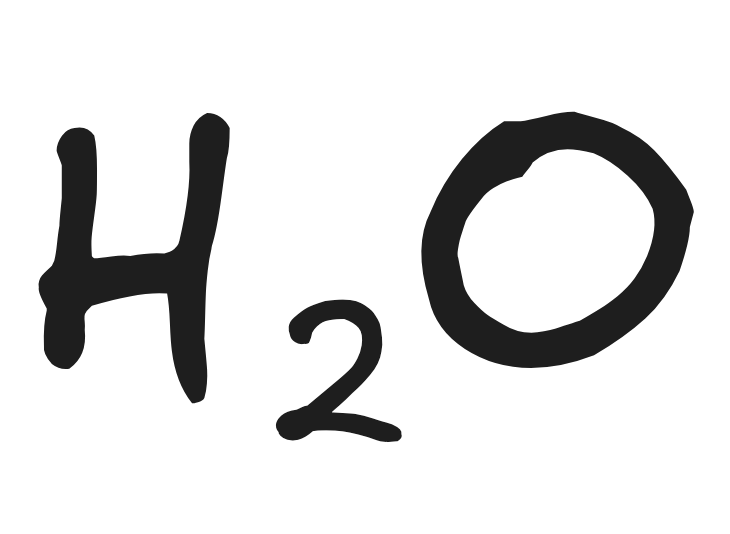
\includegraphics[width=50pt]{h2osumma.png} \hspace{2cm} 
    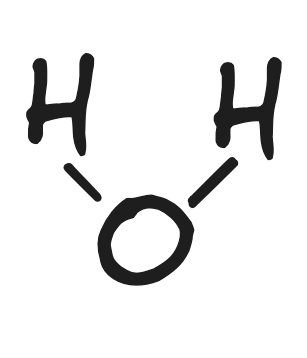
\includegraphics[width=50pt]{h2ostruktur.png} 
\end{center}
\vspace{5mm} 
\begin{center}
    \textbf{Summaformel} \hspace{3cm} \textbf{Strukturformel}
\end{center}

\vspace{5mm} 
\hrule 
\vspace{5mm} 

\question Vad \textbf{heter ämnena} och vad kallas den \textbf{typen av ämne}? (2 poäng) (Bilderna på frågan ovan)


\end{questions}

\end{document}
